\documentclass[a4paper,11pt]{article}
\input{/home/tof/Documents/Cozy/latex-include/preambule_lua.tex}
\newcommand{\showprof}{show them}  % comment this line if you don't want to see todo environment
\fancyhead[L]{arbre binaire -image}
\newdate{madate}{10}{09}{2020}
%\fancyhead[R]{\displaydate{madate}} %\today
%\fancyhead[R]{Seconde - SNT}
%\fancyhead[R]{Première - NSI}
\fancyhead[R]{Terminale - NSI}
\fancyfoot[L]{~\\Christophe Viroulaud}
\AtEndDocument{\label{lastpage}}
\fancyfoot[C]{\textbf{Page \thepage/\pageref{lastpage}}}
\fancyfoot[R]{\includegraphics[width=2cm,align=t]{/home/tof/Documents/Cozy/latex-include/cc.png}}

\begin{document}
\begin{Form}
\begin{center}
\begin{tikzpicture}
\node[draw] (A) at (0,0) {A};
\node[draw] (B) at (-3,-1) {B};
\node[draw] (C) at (-5,-2) {C};
\node[draw] (D) at (-1,-2) {D};
\node[draw] (E) at (-6,-3) {E};
\node[draw] (F) at (-4,-3) {F};
\node[draw] (H) at (-2,-3) {H};
\node[draw] (I) at (3,-1) {I};
\node[draw] (J) at (2,-2) {J};
\node[draw] (K) at (4,-2) {K};
\node[draw] (L) at (5,-3) {L};
\draw (A) -- (B);
\draw (C) -- (B);
\draw (C) -- (E);
\draw (C) -- (F);
\draw (D) -- (B);
\draw (D) -- (H);
\draw (A) -- (I);
\draw (J) -- (I);
\draw (I) -- (K);
\draw (L) -- (K);
\end{tikzpicture}
\captionof{figure}{Un arbre binaire équilibré non complet}
\label{arbre}
\end{center}
\begin{center}
\begin{tikzpicture}
\node[draw] (A) at (0,0) {A};
\node[draw] (B) at (-3,-1) {B};
\node[draw] (C) at (-5,-2) {C};
\node[draw] (D) at (-1,-2) {D};
\node[draw] (E) at (-6,-3) {E};
\node[draw] (F) at (-4,-3) {F};
\node[draw] (H) at (-2,-3) {H};
\node[draw] (I) at (3,-1) {I};
\node[draw] (J) at (0, -3) {J};
\node[draw] (K) at (4,-2) {K};
\node[draw] (L) at (5,-3) {L};
\draw (A) -- (B);
\draw (C) -- (B);
\draw (C) -- (E);
\draw (C) -- (F);
\draw (D) -- (B);
\draw (D) -- (H);
\draw (A) -- (I);
\draw (J) -- (D);
\draw (I) -- (K);
\draw (L) -- (K);
\end{tikzpicture}
\captionof{figure}{Un arbre binaire non équilibré}
\label{arbre}
\end{center}
\begin{center}
\begin{tikzpicture}
\node[draw] (A) at (0,0) {A};
\node[draw] (B) at (-3,-1) {B};
\node[draw] (C) at (-5,-2) {C};
\node[draw] (D) at (-1,-2) {D};
\node[draw] (E) at (-6,-3) {E};
\node[draw] (F) at (-4,-3) {F};
\node[draw] (H) at (-2,-3) {H};
\node[draw] (I) at (3,-1) {I};
\node[draw] (J) at (2,-2) {J};
\node[draw] (K) at (4,-2) {K};
\node[draw] (L) at (0,-3) {L};
\draw (A) -- (B);
\draw (C) -- (B);
\draw (C) -- (E);
\draw (C) -- (F);
\draw (D) -- (B);
\draw (D) -- (H);
\draw (A) -- (I);
\draw (J) -- (I);
\draw (I) -- (K);
\draw (L) -- (D);
\end{tikzpicture}
\captionof{figure}{Un arbre binaire complet}
\label{arbre}
\end{center}
\begin{center}
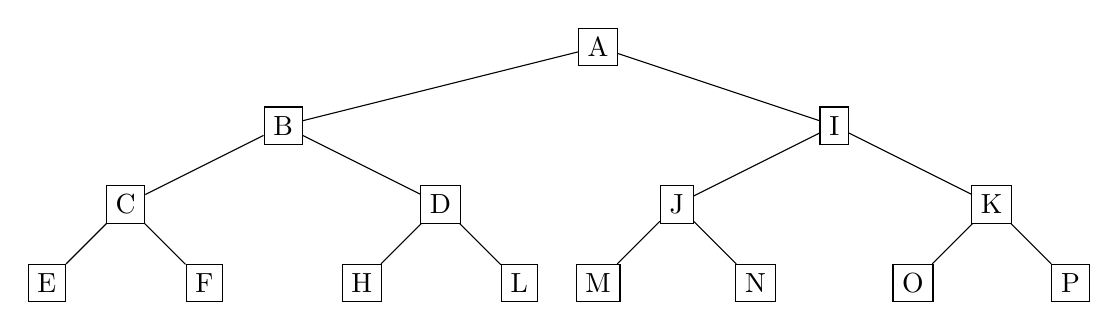
\begin{tikzpicture}
\node[draw] (A) at (1,0) {A};
\node[draw] (B) at (-3,-1) {B};
\node[draw] (C) at (-5,-2) {C};
\node[draw] (D) at (-1,-2) {D};
\node[draw] (E) at (-6,-3) {E};
\node[draw] (F) at (-4,-3) {F};
\node[draw] (H) at (-2,-3) {H};
\node[draw] (I) at (4,-1) {I};
\node[draw] (J) at (2,-2) {J};
\node[draw] (K) at (6,-2) {K};
\node[draw] (L) at (0,-3) {L};
\node[draw] (M) at (1,-3) {M};
\node[draw] (N) at (3,-3) {N};
\node[draw] (O) at (5,-3) {O};
\node[draw] (P) at (7,-3) {P};

\draw (A) -- (B);
\draw (C) -- (B);
\draw (C) -- (E);
\draw (C) -- (F);
\draw (D) -- (B);
\draw (D) -- (H);
\draw (A) -- (I);
\draw (J) -- (I);
\draw (I) -- (K);
\draw (L) -- (D);
\draw (J) -- (M);
\draw (J) -- (N);
\draw (K) -- (O);
\draw (K) -- (P);
\end{tikzpicture}
\captionof{figure}{Un arbre binaire parfait}
\label{arbre}
\end{center}
\begin{center}
\begin{tikzpicture}
\node[draw] (A) at (0,0) {A};
\node[draw] (B) at (-1,-1) {B};
\node[draw] (C) at (-2,-2) {C};
\node[draw] (D) at (-3,-3) {D};

\draw (A) -- (B);
\draw (C) -- (B);
\draw (C) -- (D);
\end{tikzpicture}
\captionof{figure}{Un arbre binaire minimal}
\label{arbre}
\end{center}
\end{Form}
\end{document}